\section{Framework}
\label{architecture_s}	
Figure~\ref{architecture} presents the proposed overall architecture for ensuring Java bytecode correctness. 

\begin{figure}[!tbp]
\begin{center}
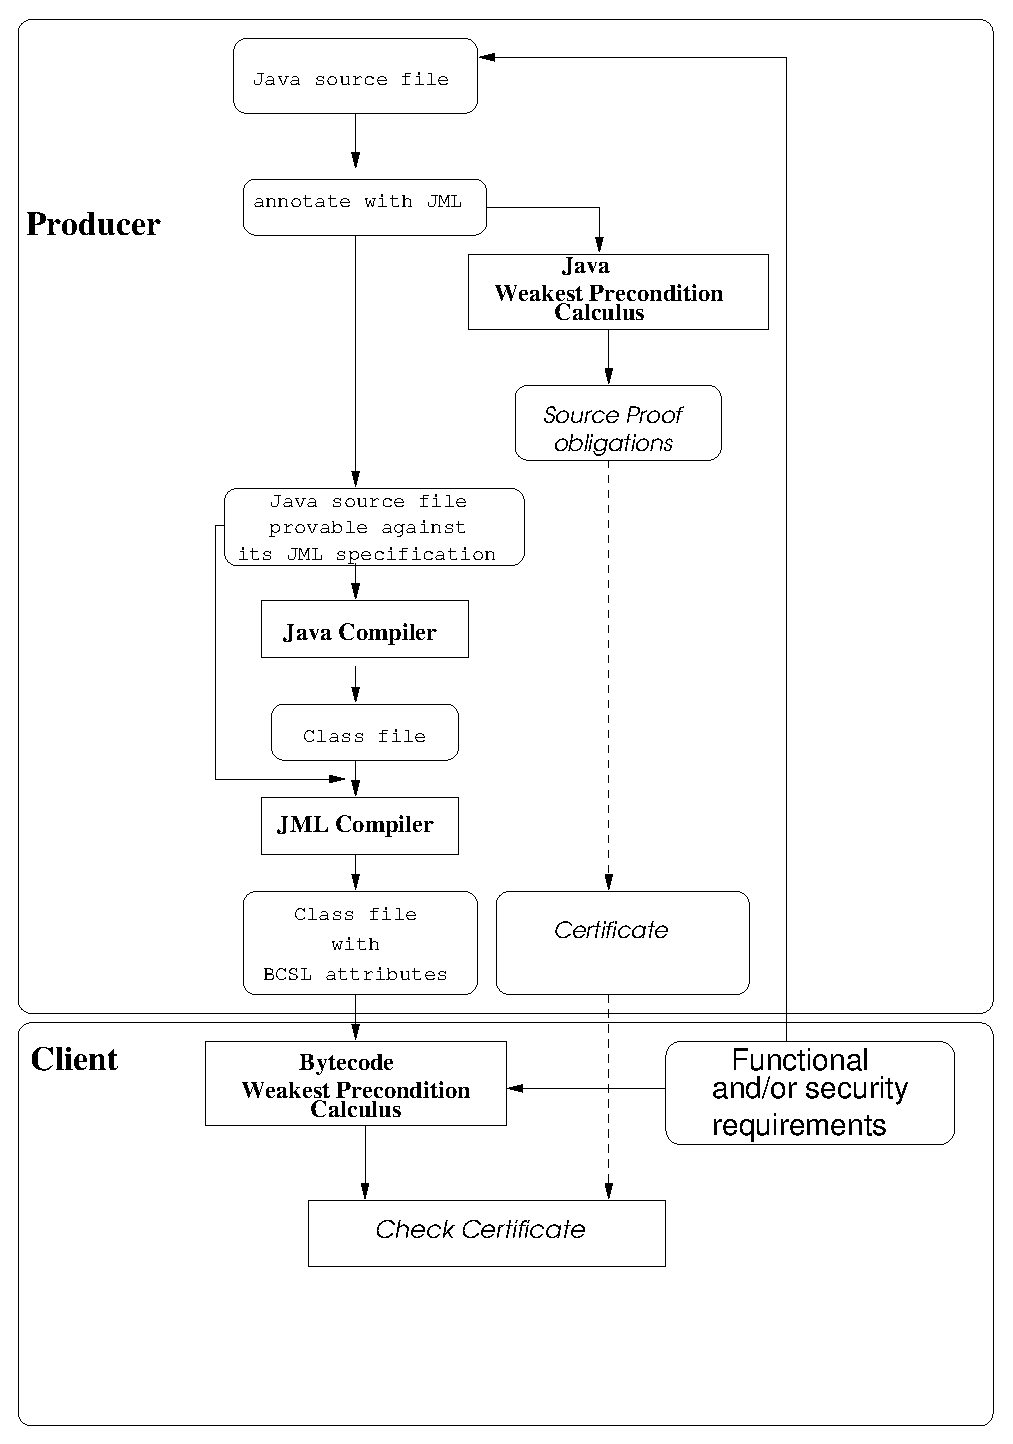
\epsfig{file=architecture.eps, width=\linewidth}
\caption{The overall architecture for annotating and verifying code}
\label{architecture}
\end{center}
\end{figure}
%\clearpage

It describes a process that allows a client to trust a code produced by an untrusted code producer. This approach is especially suitable
 in cases where the client policy involves non trivial functional or safety requirements and thus, an automatic specification inference cannot be applied.

In the first stage of the process the client provides the functional and (or) security requirements to the producer.
 The requirements can be in different form:
\begin{itemize}
\item A specified interface that describes the application to be developed. In that case,
 the client specifies in JML the features that have to be implemented by the code producer.
\item An API with restricted access to some method. In this case, the client can protect its system by restricting the API usage.
For example, suppose that the client API provides transaction management facilities - the API method \texttt{open} for opening and method \texttt{close} for closing transactions. In this case, a requirement can be for no nested transactions.
In this case, the methods \texttt{open} and \texttt{close} can be annotated to ensure that the method \texttt{close} 
 should not be called if there is no transaction running and the method \texttt{open} should not be called if there is already a running transaction. In this scenario we can apply results of previous work \cite{PBBHL}.  
\end{itemize}

%OLD:
% In the development process, the producer uses Jack to check the client requirements and usually has to add JML annotations for this %In both cases, the code producer develops its application and proves that it fulfills the given requirements using Jack; %in most cases, to complete this task, some annotations have to be added to the code 
%e.g. loop invariants, class invariants, method preconditions and postconditions etc. In a standard, application only after specifying enough the source code, 
%have we got the annotated Java source files to feed to the JML compiler.

In the development process, the producer verifies if the client requirements are respected by generating verification conditions
over the source code and usually, he has to add JML annotations for this e.g. loop invariants, class invariants, method preconditions
 and postconditions etc. It is usually only after specifying enough the source code that the annotated Java source and class files are fed to the JML compiler.
% Usually, only after ``specifying enough'' the source code, 
%have we got the annotated Java source files to feed to the JML compiler.

If the annotations are sufficient to prove the code, 
the Java file is normally compiled with a Java compiler to obtain a 
class file. This class file is then extended with user defined attributes that contain the BCSL specification, 
resulting from the compilation of the JML specification in the Java source file. 
At this stage, the Java class files contain all the information that will allow the client to check if the bytecode does not violate 
his requirements. 
 %OLD
%In particular, the client will generate proof obligations from the untrusted annotated bytecode and his security requirements 
%(expressed in a suitable form) as shown in figure~\ref{architecture}. Proof obligations are formulas which, if provable, guarantee the bytecode correctness.
%The latter are then proved , for instance, with JACK (see section \ref{prelim}). If the client succeeds in proving 
%the verification conditions, he can trust the unknown code. Currently the framework does not support sending both the proof and the 
%bytecode to the client, which is the next step in our work.
In particular, the client will generate proof obligations from the untrusted annotated bytecode and his security requirements 
(expressed in a suitable form) as shown in figure~\ref{architecture}. Proof obligations are formulas which, if provable, guarantee the bytecode correctness.
The latter are then proved with a theorem prover (possibly interactively). If the client succeeds in proving 
the verification conditions, he can trust the unknown code. 

Currently the framework does not support sending both the proof and the 
bytecode to the client this being the next step in our work. 

%Actually, our early experiments show that the proof obligations on source and bytecode level are syntactically modulo names and types.   

%OLD
%To implement this architecture, we have defined a compiler from JML to BCSL; the JML compilation results in an extension of the class file format; 
%we have implemented a tool to insert those special attributes in the class file and we have extended the JACK framework to generate proof obligations at bytecode 
%level and to prove them with the plugged JACK provers (as explained in the introduction). 
%The coming sections introduce those features.  

To implement this architecture we use JACK as a verification condition generator both on the consumer and the
producer side. JACK is a plugin for the eclipse\footnote{http://www.eclipse.org} integrated development environment for Java. Originally, the tool was designed as verification condition generator for Java source programs against their JML specification. JACK can interface with several theorem provers (AtelierB, Simplify, Coq, PVS). We have extended the tool with a compiler from JML to BCSL and a bytecode verification condition generator. In the following we introduce the BCSL language, the JML compiler and the bytecode weakest precondition calculus which underlines the bytecode verification condition generator.
 
%the JML compilation results in an extension of the class file format; we have implemented a tool to insert those special attributes in the class file and we have extended 
%the JACK framework to generate proof obligations at bytecode level and to prove them with the plugged JACK provers (as explained in the introduction). 
%The coming sections introduce those features.  
